% A workaround to allow relative paths in included subfiles
% that are to be compiled separately
% See https://tex.stackexchange.com/questions/153312/subfiles-inside-a-subfile-using-relative-paths
\providecommand{\main}{..}
% \documentclass[\main/thesis.tex]{subfiles}

\begin{document}
\chapter{Background on Reinforcement Learning}
\label{ch2:background}

In this chapter we introduce the notation and background knowledge necessary for the theory $n$-step $Q(\sigma)$. 
Throughout this chapter we denote random variables with upper-case letters, e.g. $X$. 
Scalar values, including those representing the realization of random variables, are denoted with lower-case letters, e.g. $x$.
Sets are denoted with an upper-case calligraphic letter, e.g. $\mathcal{X}$. 
Finally, vectors and matrices are represented with bold symbols or letters: lower-case for vectors, e.g. $\textbf{x}$, and upper-case for matrices, e.g. $\textbf{X}$.

%%%%%%%%%% RL and Finite MDP's %%%%%%%%%%
\section{Reinforcement Learning and Finite Markov Decision Processes}

Reinforcement Learning (RL) is learning how to map situations to actions in order to maximize a numerical signal.
Just like rats learn to navigate mazes to gain access to food in psychological experiments, learners, or agents,  in the RL framework learn how to act in order to gain access to a numerical signal. 
Because of its close similarity to the food or other rewards provided to animals in psychological experiments, this numerical signal is also called \textit{reward}. 
Just like the rat in the maze is not told where to go, RL agents are not given exact instructions on how to act.
Instead, agents are given a set of actions that they can use in order to gain rewards as they interact with the world.
Through the process of trial and error, agents learn to map aspects of the world to particular actions in order to maximize the reward they receive.

Formally, in RL the sequential decision making problem is formulated as a finite \textit{Markov Decision Process} (MDP).
In the MDP framework there exist two main entities - the agent and the environment.
The \textit{agent} is both a learner and a decision maker.
The \textit{environment} is everything that the agent interacts with and is external to the agent. 
The agent and the environment interact over a sequence of discrete timesteps, $t=0,1,2,...$. 
At every timestep, the agent receives information about the environment's \textit{state}, $S_t \in \mathcal{S}$, where $\mathcal{S}$ is a finite set of all possible states. 
On the basis of that information, the agent selects an \textit{action}, $A_t$, from a finite set of actions, $\mathcal{A}$.
As a function of its current state and selected action, the agent receives a real-valued random reward, $R_{t+1} = R(S_t,A_t) \in \mathcal{R} \subset \mathbb{R}$, where $\mathcal{R}$ is a finite subset of $\mathbb{R}$.
The agent then transitions to another state, $S_{t+1}$, according to the \textit{state-transition probability function}, $P$, defined as
%
\begin{equation}
\label{eq:StateTransition}
\mathbb{P}(S_{t+1} = s' | S_t = s, A_t = a) = \mathbb{P}(s'|s,a) = P^a_{ss'}, \ 
	(s,a,s') \in	\mathcal{S} \times \mathcal{A} \times \mathcal{S},
\end{equation}
where $s'$, $s$, and $a$ are the realizations of $S_{t+1}$, $S_t$, and $A_t$, respectively. 
We use the abbreviation $P^a_{ss'}$ for conciseness and only when doing so is not ambiguous.

Note that the discrete probability distribution in equation (\ref{eq:StateTransition}) is only well defined because the sets $\mathcal{S}$ and $\mathcal{A}$ are finite.
Similarly, since $\mathcal{R}$ is finite, we can define a probability distribution for the reward function $R(S_t,A_t)$ as
%
\begin{equation}
\label{eq:RewardFunc}
\mathbb{P}(R_t = r | S_t = s, A_t = a) \ \forall \ (s,a,r) \in \mathcal{S} \times \mathcal{A} \times \mathcal{R},
\end{equation}
and its expected value as
%
\begin{equation}
\label{eq:RewardEV}
\mathbb{E}_R \{ R(S_t, A_t) | S_t = a, A_t = a \} = \sum_{r \in \mathcal{R}} r \mathbb{P}(r| S_t =s, A_t=a)
	= r(s,a),
\end{equation}
where $\mathbb{E}_R$ stands for the expected value with respect to the reward function $R$.
We will use the abbreviation $r(s,a)$ only when doing so does not result in ambiguities.

%%%%% Episodic vs Continuing Tasks %%%%%
\subsection{Episodic and Continuing Tasks}

The dynamics of the MDP and the agent's actions give rise to a infinite sequence or \textit{trajectory} of states, actions and rewards
\begin{equation*}
S_0, A_0, R_1, S_1, A_1, R_2, S_2, A_2, R_3 ....
\end{equation*}
A distinguishing characteristic of MDPs is whether they ever reach a state, $s_{terminal}$, such that $\mathbb{P}(s_{terminal} | s_{terminal}, a) = 1$ and $R(s_{terminal}, a) = 0$ for all $a \in \mathcal{A}$. $S_{terminal}$ is called a \textit{zero-reward absorbing} state, or, informally, a \textit{terminal} state.
After reaching the terminal state, the agent cannot possibly gain any more reward or escape the terminal state; for example, death would be humans' terminal state.

When the MDP contains a terminal state, the trajectory of states, actions, and rewards can be rewritten as a finite trajectory
\begin{equation*}
S_0, A_0, R_1, S_1, A_1, R_2, ..., S_T,
\end{equation*}
where $T$ is the time when the agent reaches the terminal state. This is the case of MDP's that represent tasks that have a clear ending after which the agent cannot gain any more reward. A classical example of this type of tasks are board games such as Chess and Go. These type of tasks are named \textit{episodic tasks}.

On the other hand, for MDP's that represent tasks that have no clear ending, the sequence of states, actions, and rewards, continues indefinitely. These type of tasks are known as \textit{continuing tasks}.

%%%%%%%%%% Discounted Returns, Policies, and Value Functions %%%%%%%%%%
\section{Discounted Returns, Policies, and Value Functions}

The goal of reinforcement learning agents is to maximize the expected cumulative reward that they receive given the MDP dynamics. Formally, the agent looks to maximize the expected \textit{return}, where the return, denoted $G_t$, is a sum of rewards
\begin{equation}
\label{eq:return}
G_t = R_{t+1} + R_{t+2} + ... + R_T = \sum^T_{k=0} R_{t+1+k}.
\end{equation}
In the case where the environment has a terminal state, $T$ is an integer representing the time when the agent reaches the terminal state.
On the other hand, when the MDP does not have a terminal state, the sum of rewards continues indefinitely; consequently, we would take $T \rightarrow \infty$.
Since the sum of the rewards becomes intractable when there is no terminal state, we consider instead the \textit{discounted return}
\begin{equation}
\label{eq:disreturn}
G_t = R_{t+1} + \gamma R_{t+2} + \gamma^2 R_{t+3} + ... = \sum^T_{k=0} \gamma^k R_{t+1+k},
\end{equation}
where $\gamma$ is a discount factor in the half-open interval $[0,1)$ and it can be equal to $1$ only when the MDP has a terminal state. Note that $G_t$ can be written recursively in the following way
\begin{equation}
\label{eq:rec_return}
G_t = R_{t+1} + \gamma R_{t+2} + \gamma^2 R_{t+3} + ... = R_{t+1} + \gamma G_{t+1}.
\end{equation}

In order to make informed decisions, agents often use \textit{value functions} that determine how ``good'' is a state or a state-action pair. 
In this case, the ``goodness'' of states - or state-action pairs - is measured in terms of how much expected future reward the agent will gain if a trajectory starts at a given state - or state-action pair.
Since the expected future reward is determined by the agent actions, value functions are determined by the particular decision rule that the agent uses to choose actions. This decision rule is known as a \textit{policy}.

Formally, a policy is a mapping from states to a probability distribution over the actions.
We often denote policies as $\pi$ or $\mu$ and let $\pi(a|s)$ or $\mu(a|s)$ be the probability of taking action $a$ while in state $s$. 
Additionally, policies can also be a function of the time, $t$, in which case they are denoted $\pi_t$ or $\mu_t$.
Given a policy, $\pi$, the \textit{state-value} function induced by this policy is defined as
\begin{equation}
\label{eq:valuefunc}
v_\pi(s) \overset{.}{=} \mathbb{E}_{\pi, P, R} \{ G_t | S_t = s \} = 
	\mathbb{E}_{\pi, P, R} \Big\{ \sum^T_{k=0} \gamma^k R_{t+1+k} | S_t = s \Big\} 
    \ \forall \ s \in \mathcal{S}.
\end{equation}
Note that the expectation in equation (\ref{eq:valuefunc}) is with respect to the policy, $\pi$, the state transition function, $P$, and the reward function, $R$. We will omit the subscript $P$ and $R$ when doing so is not ambiguous. 

Similarly, we can define the value function with respect to state-action pairs, called \textit{action-value function}, as
\begin{equation}
\label{eq:av_func}
q_\pi(s,a) \overset{.}{=} \mathbb{E}_{\pi, P, R} \{ G_t | S_t = s, A_t = a\} 
	\ \forall \ (s,a) \in \mathcal{S} \times \mathcal{A}.
\end{equation}
It is important to note that there exist a bidirectional relationship between the state-value and the action-value function
\begin{align*}
v_\pi(s) &= \sum_{a \in \mathcal{A}} \pi(a|s) q_\pi(s,a) \\
q_\pi(s,a) &= r(s,a) + \sum_{s' \in \mathcal{S}} P^a_{ss'} v_\pi(s') \\
            &= r(s,a) + \sum_{s' \in \mathcal{S}} P^a_{ss'} \sum_{a' \in \mathcal{A}}
            \pi(a|s') q_\pi(s', a')
\end{align*}

%%%%% Bellman Equations and Backup Diagrams %%%%%
\subsection{Bellman Equations and Backup Diagrams}
\label{subsec:backup_diagrams}

Similar to the recursive return in equation (\ref{eq:rec_return}), state-value functions can also be defined recursively
\begin{align}
\label{eq:sv_bellman}
v_\pi(s) &= \mathbb{E}_\pi\{ R(S_t, A_t) + \gamma G_{t+1} | S_t = s \} \nonumber \\
%
&= \sum_{a \in \mathcal{A}} \pi(a|s) [ r(s,a) + \gamma \sum_{s' \in \mathcal{S}} P^a_{ss'} v_\pi(s') ] 
	\nonumber \\
%
&= \sum_{a \in \mathcal{A}} \sum_{s' \in \mathcal{S}} \pi(a|s) P^a_{ss'} [ r(s,a) 
	+ \gamma v_\pi(s')].
\end{align}
The same can be said for action-value functions
\begin{align}
\label{eq:av_bellman}
q_\pi(s,a) &= \mathbb{E}_\pi \{ R(S_t, A_t) + \gamma G_{t+1} | S_t = s, A_t = a \} \nonumber \\
%
&= r(s,a) + \gamma \sum_{s' \in \mathcal{S}} P^a_{ss'} \sum_{a' \in \mathcal{A}} \pi(a'|s') q_\pi(s',a')
	\nonumber \\
%
&= \sum_{s' \in \mathcal{S}} \sum_{a' \in \mathcal{A}} P^a_{ss'} \pi(a'|s') [r(s,a) + \gamma q_\pi(s',a')].
\end{align}

Equations (\ref{eq:sv_bellman}) and (\ref{eq:av_bellman}) are called \textit{Bellman equations}.
They illustrate the relationship between the value of a state - or a state-action pair - and the value of its successor states - or successor state-action pairs.

Bellman equations can be represented as \textit{backup diagrams} such as the ones in figure (\ref{fig:bellman_backup}).
Backup diagrams are useful to provide high level intuition about how information flows from successor states to the current state.
This will be particularly useful  in the next section when we introduce ways to estimate the state-value and action-value functions.

Figure (\ref{fig:bellman_backup}a) shows the backup diagram of the bellman equation in (\ref{eq:sv_bellman}).
Empty circles represent states, whereas solid ones represent actions.
Branches leading from states are weighted according to the policy, $\pi$.
Branches connecting actions with states are weighted according to the state-transition function, $P$, and are associated with an expected reward, $r$. 
In the case of the backup diagram for the action-value functions in figure (\ref{fig:bellman_backup}b), branches and circles have the same meaning, except for the root of the diagram which represents the initial state-action pair.

\begin{figure}
    \centering
    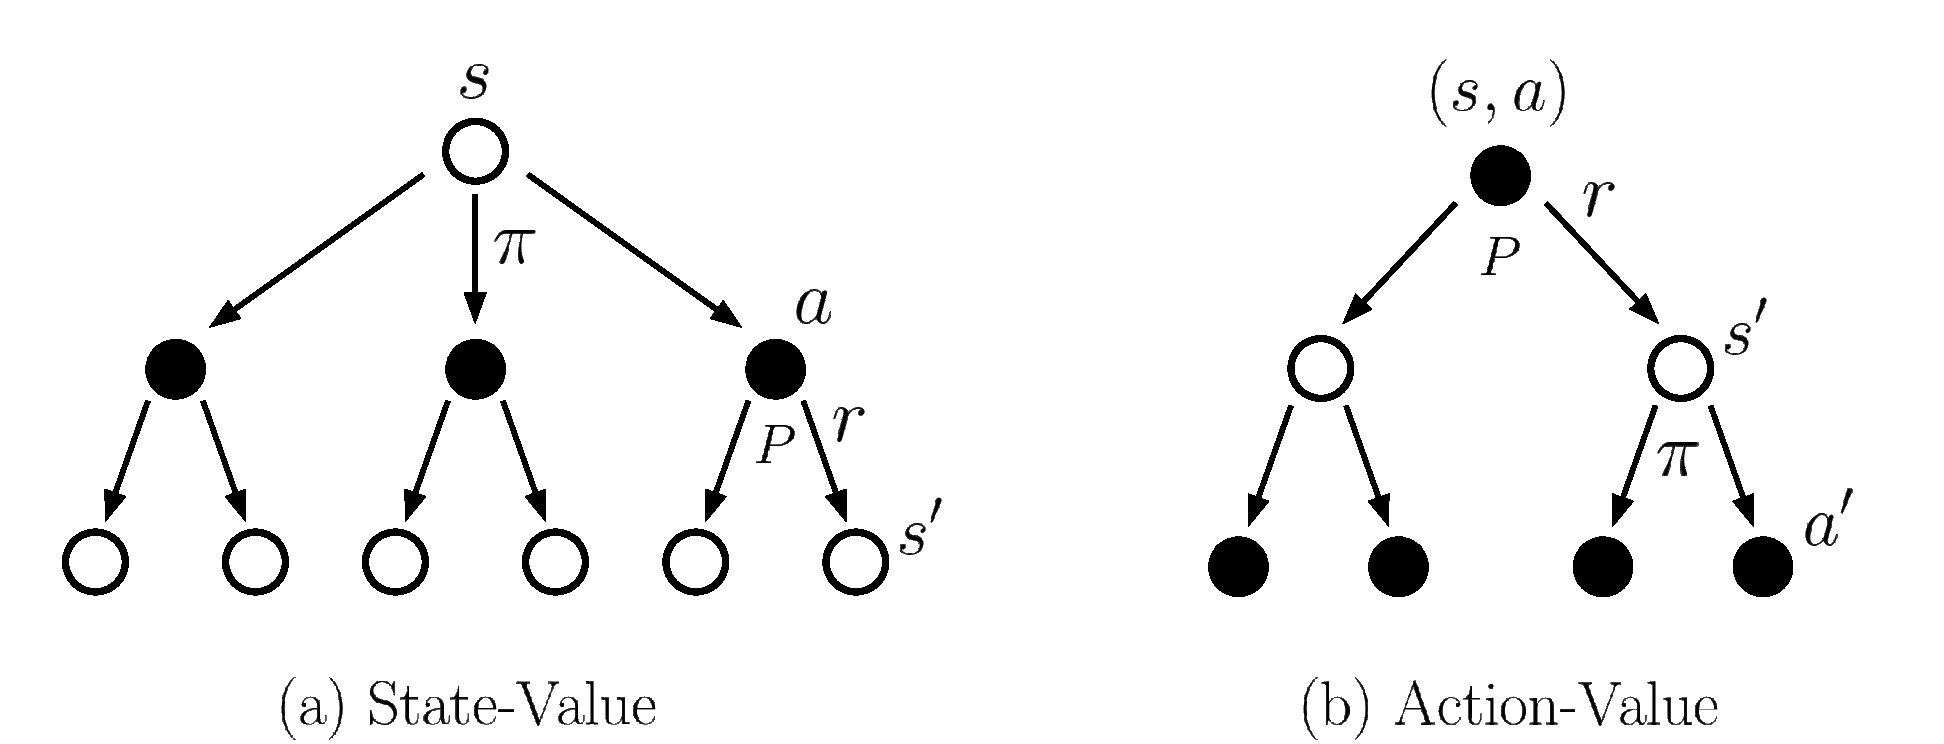
\includegraphics[keepaspectratio=true, width=1\textwidth]{\main/img/bellman_backup.pdf}
    \caption[Backup Diagrams for Bellman Equations] {Backup Diagrams for Bellman Equations. 
    (a) Backup diagram for the Bellman equation corresponding to the state-value function.
    (b) Backup diagram for the Bellman equation corresponding to the 
    action-value function.}
    \label{fig:bellman_backup}
    % Put the label *after* the caption, but inside the float
\end{figure}


%%%%% Optimal and Exploratory Policies %%%%%
\subsection{Optimal and Exploratory Policies}

As discussed above, the goal of an RL agent is to maximize the amount of expected reward that it will receive. 
This is equivalent to finding a policy, $\pi_*$, such that the expected return that it generates is greater than or equal to the expected return of any other policy.
We call $\pi_*$ an \textit{optimal policy}.

Finite MDP's can have several optimal policies.
However, all optimal policies share the same value functions.
The state-value function induced by an optimal policy $\pi_*$, denoted $v_*$, is called \textit{optimal state-value function} and is defined as
%
\begin{equation}
\label{eq:optimal_svfunc}
v_*(s) \overset{.}{=} \max_\pi v_\pi (s) 
	= \mathbb{E}_{\pi_*}\{ \max_a R(S_t, a) + \gamma v_*(S_{t+1}) | S_t = s \}.
\end{equation}
Similarly, the action-value function corresponding to an optimal policy is defined as 
%
\begin{equation}
\label{eq:optimal_avfunc}
q_*(s,a) \overset{.}{=} \max_\pi q_\pi(s,a) 
	= \mathbb{E}_{\pi_*} \{R_{t+1} + \gamma \max_{a'} q_*(S_{t+1}, a') | S_t = s, A_t =a \}
\end{equation}

$\pi_*$ is a special case of a \textit{greedy policy} because it selects an action that maximizes the action-value $q_*$. 
Since $q_*$ is the optimal action-value function, $\pi_*$ is guaranteed to be optimal.
In the case where $q_*$ is not available, an agent often uses an estimate, $Q$, of $q_*$.
In this case behaving greedily with respect to $Q$ does not guarantee that the corresponding policy will be optimal. 
Moreover, since the algorithms for estimating $q_\pi$ require that every state-action pair is observed an infinite amount of time, behaving greedily with respect to $Q$ often hinders convergence to $q_*$.

Instead of behaving greedily, agents behave according to \textit{exploratory policies} that guarantee that every state-action pair is going to be observed enough times to guarantee convergence.
One example of exploratory policies are $\epsilon$\textit{-greedy} policies, a simple kind of exploratory policies where the greedy action is selected with probability $1-\epsilon$, otherwise, a random action is selected. 
In this case, $\epsilon$ is an exploration parameter in the interval $[0,1]$ that controls the degree of ``greediness" of the policy. 

% Another example of an exploratory policy is \textit{Boltzmann exploration} where actions are selected according to the probability distribution
% \begin{equation}
% \label{eq:boltzmann_exp}
% \mathbb{P}(a|s,t,Q) = \frac{e^{\beta_t(s) Q(s,a)}}{\sum_{a' \in \mathcal{S}} e^{\beta_t(s) Q(s,a)}},
% \end{equation}
% where $Q$ is the current estimate of the action-value function, $t$ is the current timestep, and $\beta_t(s)$ is a state-specific exploration parameter in the interval 

%%%%%%%%%% Estimating Value Functions %%%%%%%%%%
\section{Temporal-Difference Methods}

One of the main challenges in RL is estimating value functions as the agent is interacting with the environment.
\textit{Temporal-difference} (TD) methods are a type of prediction method used to compute new estimates of the value function by using old estimates, a technique known as \textit{bootstrapping}.
TD methods compute value functions using \textit{update functions} of the form
\begin{align}
\label{eq:val_func_update}
\text{New Estimate} & = \text{Old Estimate} 
	+ \alpha [\text{Target Estimate} - \text{Old Estimate}] \nonumber \\
%
& = (1-\alpha) \ \text{Old Estimate} + \alpha \ \text{Target Estimate},
\end{align}
where $\alpha$ is a learning rate parameter in the half-open interval $(0,1]$.

% and the $\leftarrow$ indicates that the new estimate is being assigned the value on the right-hand side of the equation.

In essence, the new estimate of the value function is computed using a moving average between the old estimate and the target estimate.
As iterations continue, the estimate of the value function moves closer and closer to the target estimate.
The target estimate that we use is the expected discounted return given the current state or state-action pair, depending on the type of value function.
The discounted return can be estimated by sampling sequences of rewards until an episode terminates.
This is analogous to Monte Carlo estimation methods where trajectories are simulated and an estimate is computed from averaging over a large number of trajectories.
However, this approach is infeasible in continuing tasks and, even in episodic tasks, is highly inefficient. 

TD methods take an alternative approach. 
Instead of sampling a trajectory of rewards, one can sample one reward and the next value or action-value function after that. 
For example, when estimating $v_\pi(S_t)$ one can use $R(S_t, A_t) + \gamma v_\pi(S_{t+1})$ as an estimate because in expectation it is equal to $v_\pi(S_t)$.
% \begin{equation*}
% \mathbb{E}_\pi \{ R(S_t,A_t) + \gamma v_\pi(S_{t+1}) | S_t \} = v_\pi(S_t).
% \end{equation*}
However, since we do not have access to $v_\pi(S_t)$, we use $V_t(S_t)$ instead as an approximation.
Therefore, when computing the estimate of the state-value function we can use the update rule 
\begin{equation}
\label{eq:td0_update}
V_{t+1} (S_t) = (1-\alpha) V_t(S_t) + \alpha [R(S_t, A_t) + \gamma V_t(S_{t+1})],
\end{equation}
where $V_{t}$ corresponds to the estimate of $v_\pi$ at time $t$ and for all the other states, $s \neq S_t$, we consider $V_{t+1}(s) = V_{t}(s)$.

The update function in equation (\ref{eq:td0_update}) corresponds to the algorithm TD(0) (\cite{sutton1988learning}) and is used to compute estimates of the state-value function as the agent is interacting with its environment.
It is possible to use stochastic approximation theory to prove that the estimates computed by the TD(0) algorithm with state and action specific learning rates, i.e. $\alpha(S_t,A_t)$, converge to $v_\pi$ (\cite{Bertsekas:1996:NP:560669}). 

%%%%% Action-Value Methods %%%%%
\subsection{Action-Value Methods}
\label{subsec:av_methods}

Similar to state-value functions, we can use the update rule in (\ref{eq:val_func_update}) and a truncated estimate of the discounted return to compute new estimates of the action-value function.
In this case, we use $R(S_t,A_t) + \gamma q_\pi(S_{t+1}, A_{t+1})$ as a target estimate.
Once again, if we take the expectation of this target with respect to the policy $\pi$ and condition on the initial state-action pair, we would obtain $q_\pi(S_t,A_t)$.
Since we don't have access to $q_\pi$, we use $Q_t$, the current estimate of the action-value function, as an approximation.
Hence, we obtain the following update rule
\begin{align}
\label{eq:sarsa_update}
Q_{t+1}(S_t,A_t) & = Q_t(S_t,A_t) + \alpha [R(S_t, A_t) 
	+ \gamma Q_t(S_{t+1}, A_{t+1}) - Q_t(S_t, A_t)] \nonumber \\
%
& = (1-\alpha) Q_t(S_t, A_t) + \alpha [R(S_t, A_t) + \gamma Q_t(S_{t+1}, A_{t+1})] \nonumber \\
%
& = (1-\alpha) Q_t(S_t, A_t) + \alpha \hat{G}_{t},
\end{align}
where $Q_t$ is the estimate of the action-value function at time $t$, and we let $Q_{t+1}(s,a) = Q_t(s,a)$ for all the state-action pairs not equal to $(S_t,A_t)$.
Additionally, we have denoted  the estimate of the discounted return as $\hat{G}_t$.

The update function in equation (\ref{eq:sarsa_update}) corresponds to the classical algorithm Sarsa (\cite{rummery1995,sutton1996}).
Sarsa has been shown to converge to the optimal action-value function, $q_*$, for state and action dependent learning rate, $\alpha(S_t,A_t)$, and when the policy $\pi_t$ becomes greedy in the limit and has infinite exploration (\cite{Singh2000}).

The update functions of TD methods are characterized by their estimate of the return, $\hat{G}_t$.
In fact, it is straightforward to define different algorithms for estimating action-value functions by substituting $\hat{G}_t$ in equation (\ref{eq:sarsa_update}).
For example, if we let
\begin{equation}
\label{eq:expsarsa_return}
\hat{G}^{ES}_t = R(S_t, A_t) + \gamma \sum_{a \in \mathcal{A}} \pi(a|S_{t+1}) Q_t(S_{t+1},a),
\end{equation}
and substitute $\hat{G}_t$ with $\hat{G}^{ES}_t$ in equation (\ref{eq:sarsa_update}), we obtain the update rule of the algorithm Expected Sarsa (\cite{precup2000,harm-hado-expected-sarsa})
\begin{align}
\label{eq:expsarsa_update}
Q_{t+1}(S_t, A_t) &= (1-\alpha) Q_t(S_t,A_t) + \alpha \hat{G}^{ES}_t \nonumber \\
%
&= (1-\alpha) Q_t(S_t,A_t) + \alpha [R(S_t,A_t) 
	+ \gamma \sum_{a \in \mathcal{A}} \pi(a|S_{t+1}) Q(S_{t+1},a)]. % \nonumber \\
%
% &= (1-\alpha) Q_t(S_t, A_t) + \alpha[R(S_t,A_t) + \gamma V_{t+1}].
\end{align}

Expected Sarsa takes an expectation over all the possible values of the action-value function instead of sampling the next action-value function.
Additionally, Expected Sarsa has smaller variance than Sarsa while retaining the same convergence guarantees and bias \parencite{harm-hado-expected-sarsa}.

%%%%% Off-Policy Methods %%%%%
\subsection{Off-Policy Methods}
\label{subsec:offpolicy_methods}

So far we have considered the case where the policy whose value function is being estimated, known as the \textit{target policy} and denoted $\pi$, is the same as the policy generating the behaviour, known as the \textit{behaviour policy} and denoted $\mu$.
This case is also known as the \textit{on-policy} case. 
In this section we will consider a more general case where target and behaviour policy need not to be the same, known in the literature as the \textit{off-policy} case. 

The main issue when working in the off-policy case is that the expected value of the estimate of the discounted return, $G_t$, is taken with respect to the behaviour policy, $\mu$.
In this case, $E_\mu \{ \hat{G} | S_t, A_t \}$ might not be equal to the target estimate $\mathbb{E}_\pi \{G_t| S_t, A_t \}$.
Consequently, the estimates of the value function are not guaranteed to converge to $q_\pi$.

Some algorithms are already well suited to handle this kind of scenario.
For example, the popular off-policy algorithm $Q$-Learning is able to learn the optimal action-value functions by bootstrapping on the maximum  over the actions of the next estimate action-value function \parencite{watkins1989qlearn,watkins1992}.
This results in the following update rule
\begin{align}
\label{eq:qlearning_update}
Q_{t+1}(S_t,A_t) &= (1-\alpha) Q_t(S_t, A_t) + \alpha [R(S_t, A_t) + \gamma \max_{a'} Q_t(S_{t+1}, a')]
	\nonumber \\
%
&= (1-\alpha) Q_t(S_t, A_t) + \alpha \hat{G}^{QL}_t
\end{align}

Note that if we take the expected value of $G^{QL}_t$ with respect to the behaviour policy $\mu$, we obtain
\begin{align*}
& \mathbb{E}_{\mu,P,R} \{ R(S_t,A_t) + \gamma \max_{a'} Q_t(S_{t+1}, a') | S_t = s, A_t = a \}
	\nonumber \\
%
& \hspace{120pt} = r(s, a) + \gamma \sum_{s' \in \mathcal{S}} P^a_{ss'} 
	\sum_{b \in \mathcal{A}} \mu(b|s') \max_{a'} Q_t(s',a')
	\nonumber \\
%
& \hspace{120pt} = r(s, a) + \gamma \sum_{s' \in \mathcal{S}} P^a_{ss'} \max_{a'} Q_t(s',a')
	\nonumber \\
%
& \hspace{120pt} \approx r(s,a) + \gamma \sum_{s' \in \mathcal{S}} P^a_{ss'} \max_{a'} q_*(s',a')
	\nonumber \\
%
& \hspace{120pt} = q_*(s,a),
\end{align*}
which demonstrates that, in expectation, the estimate of the return used by the $Q$-Learning algorithm is approximately equal to the action-value function that it is attempting to estimate.
In fact, this is often a necessary (but not a sufficient) condition for an off-policy algorithm to converge.
The $Q$-Learning algorithm has been proven to converge in multiple settings in RL \parencite{watkins1992,Tsitsiklis1994, Jaakkola:1994:CSI:1362288.1362296}.

Similar to $Q$-Learning, Expected Sarsa is also capable of learning off-policy without any modification \parencite{precup2000}.
In contrast, the Sarsa algorithm needs to be extended to use importance sampling in order to be able to converge in the off-policy case \parencite{precup2000}. 
The resulting estimate of the return used in the update function is
\begin{align}
\label{eq:offpolicy_sarsa_return}
\hat{G}_t &= R(S_t,A_t) + \gamma \frac{\pi(A_{t+1}|S_{t+1})}{\mu(A_{t+1}|S_{t+1})} 
    Q_t(S_{t+1}, A_{t+1}) \nonumber \\
%
&= R(S_t, A_t) + \gamma \rho_{t+1} Q_t(S_{t+1}, A_{t+1}).
\end{align}

It is straightforward to demonstrate that the the estimate of the return in (\ref{eq:offpolicy_sarsa_return}) approximates in expectation the action-value function $q_\pi$.

%%%%% Backup Diagrams for Temporal Difference Methods %%%%%
\subsection{Backup Diagrams for Temporal Difference Methods}

Just like we gave a graphical representation to Bellman equations in subsection \ref{subsec:backup_diagrams}, TD methods can also be represented as backup diagrams.
In this case, the backup diagram corresponds to the main the defining characteristic of a TD method: the estimate of the return $\hat{G}_t$.
Just as before, we let empty circles represent states, solid circles represent actions, and, in the case of the backup for action-value methods, we let the root of the backup correspond to a state-action pair.
However, note that the backup now corresponds to a single trajectory instead of an expectation over all possible states and actions.
Figure \ref{fig:td_backups} show the backup diagrams of TD(0), Sarsa, Expected Sarsa, and $Q$-Learning, respectively. 
In the case of $Q$-Learning, the arc connecting the branches corresponding to the actions represents the maximum over all the actions.
On the other hand, in the backup diagram of Expected Sarsa, the branches connecting the state to the actions are weighted by the target policy $\pi$. 

\begin{figure}
    \centering
    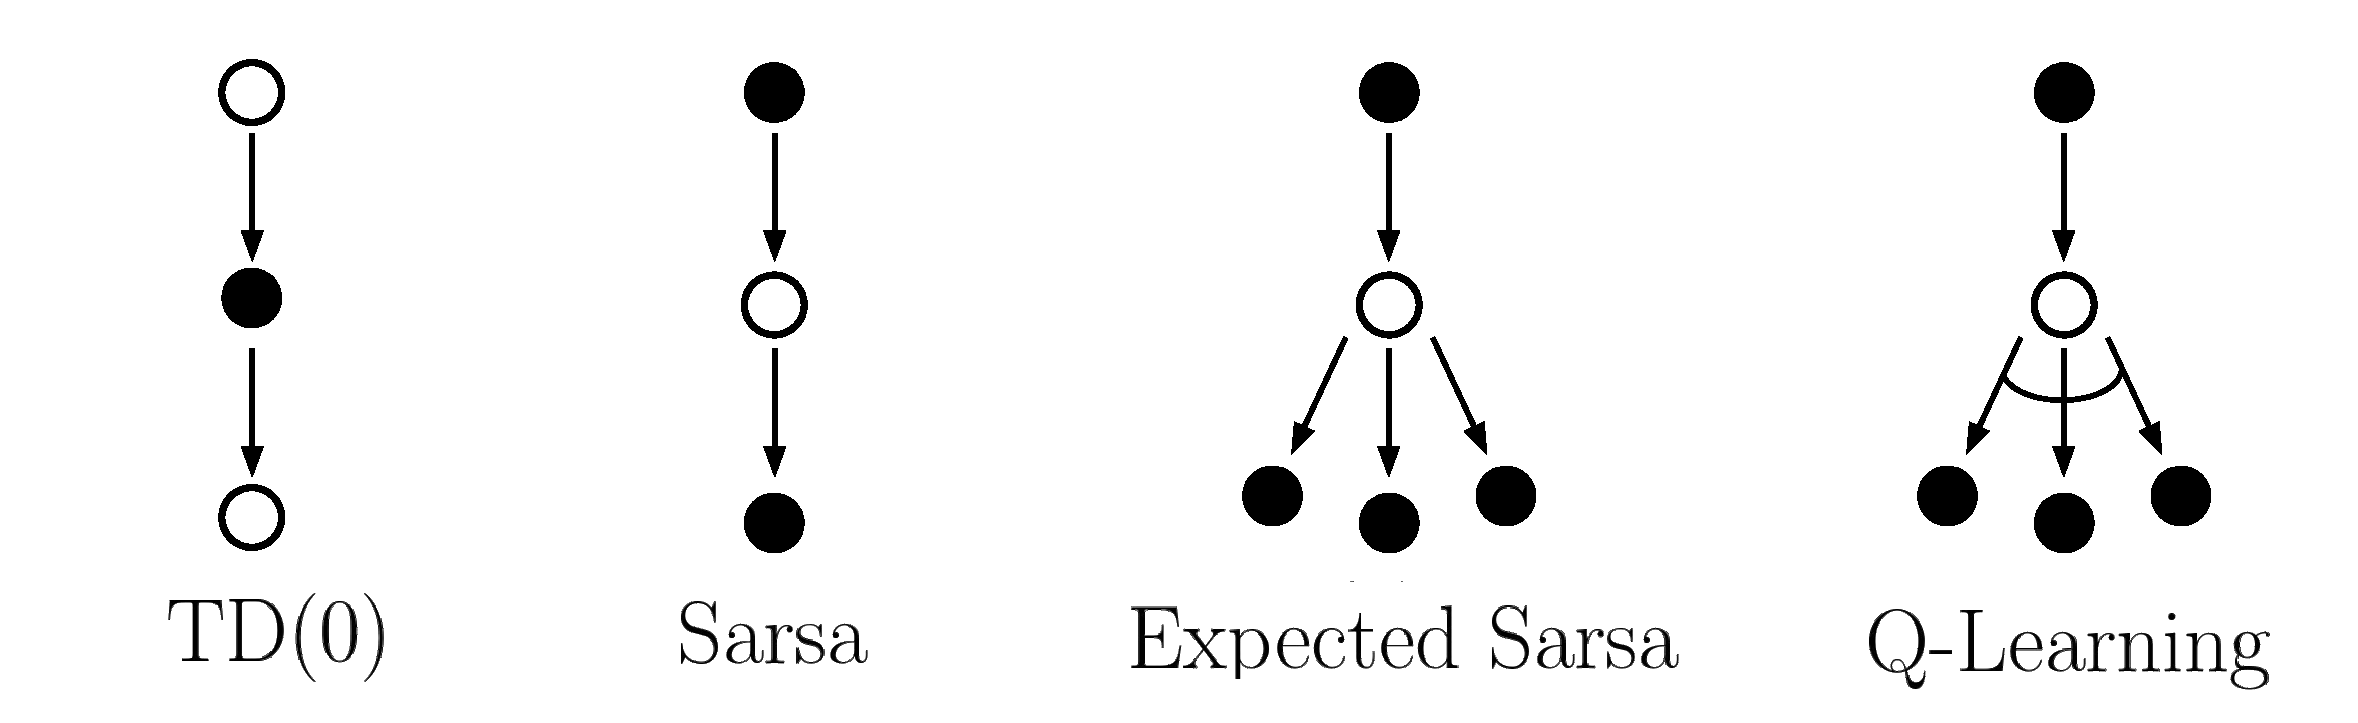
\includegraphics[keepaspectratio=true, width=1\textwidth]{\main/img/td_methods_backups.pdf}
    \caption[Backup Diagrams of TD(0), Sarsa, Expected Sarsa, and $Q$-Learning] {Backup diagrams of TD(0), Sarsa, Expected Sarsa, and $Q$-Learning.}
    \label{fig:td_backups}
    % Put the label *after* the caption, but inside the float
\end{figure}


% We will use this backup diagrams to provide a more intuitive explanation of multi-step methods in the next section.

%%%%%%%%%% n-Step Temporal Difference Methods %%%%%%%%%%
\section{n-Step Temporal Difference Methods}

In the previous section we have introduced the idea of bootstrapping in order to truncate the discounted return after one timestep.
However, we can generalize this idea to longer time intervals were instead of bootstrapping after one timestep, we bootstrap at the end of a trajectory of length $n$, where $n$ could be greater than one.
Hence, instead of using $R(S_t,A_t) + \gamma q_\pi(S_{t+1},A_{t+1})$ as a target estimate of the state-value function, we use
\begin{equation}
\label{eq:nstep_return}
G_{t:t+n} = R_{t+1} + \gamma R_{t+2} + ... + \gamma^{n-1} R_{t+n} + \gamma^n q_\pi(S_{t+n}, A_{t+n}).
\end{equation}
Note that we have used $t:t+n$ as subscripts of $G$ to denote the length of the return.
We will be using this notation henceforth.

This special case where we use a return of length $n$ as an estimate of $q_\pi$ is also known as the $n$\textit{-step} case.
Once again, if we take the expected value of the return in equation (\ref{eq:nstep_return}), we obtain $q_\pi(S_t, A_t)$ - the quantity that we are attempting to estimate.
Hence, it is still a valid estimate of the return.
Additionally, the parameter $n$ allows us to trade off bias for variance, which can potentially improve the learning performance of an algorithm \parencite{Kearns:2000:BEB:648299.755183}.

It is possible to extend Sarsa and Expected Sarsa to the $n$-step case \parencite{rummery1995,precup2000,sutton2018}.
We will be working with the general update rule
\begin{equation}
\label{eq:general_nstep_update}
Q_{t+n}(S_t, A_t) = (1-\alpha)Q_{t+n-1}(S_t,A_t) + \alpha \hat{G}_{t:t+n},
\end{equation}
where $\hat{G}_{t:t+n}$ is the estimate of the $n$-step return.
Note that the update is applied $n$ steps after the initial state-action pair was observed because only then the data needed for computing the estimate of the return is available.
Just like in the one-step case, $n$-step algorithms are characterized by their estimate of the $n$-step return $\hat{G}_{t:t+n}$.

Sarsa can easily be extended to the $n$-step case by substituting $q_\pi$ with $Q_{t+n}$ in equation (\ref{eq:nstep_return})
\begin{align}
\label{eq:nstep_sarsa}
\hat{G}^S_{t:t+n} &= R_{t+1} + \gamma R_{t+2} + \gamma^2 R_{t+3} +  ... + \gamma^n Q_{t+n-1}(S_{t+n}, A_{t+n}) 
	\nonumber \\
%
&= R_{t+1} + \gamma \hat{G}^S_{t+1:t+n}.
\end{align}
An update rule can be obtained by plugging in the $n$-step Sarsa estimate of the return into the general update rule equation (\ref{eq:general_nstep_update}).
Note that the $n$-step estimate of the return can be written recursively as in the second equality of equation (\ref{eq:nstep_sarsa}) where the base case, $G^S_{t+n:t+n}$, is defined as $Q_{t+n-1}(S_{t+n}, A_{t+n})$.
Moreover, $n$-step returns can also be represented as backup diagrams.
\textbf{Figure 1c} shows the backup diagram of the $3$-step Sarsa return. 
Additionally, $n$-step Sarsa can be extended to work off-policy by using importance sampling.
The resulting estimate of the return is
\begin{align}
\label{eq:offpolicy_nstep_sarsa}
\hat{G}^S_{t:t+n} &= R_{t+1} + \gamma \rho_{t+1} R_{t+2} + \gamma^2 \rho_{t+1} \rho_{t+2} R_{t+3} +  ... 
	\nonumber \\
&\hphantom{=}
	+ \gamma^n \big(\prod^n_{k=1} \rho_{t+k} \big) Q_{t+n-1}(S_{t+n}, A_{t+n}) 
	\nonumber \\
%
&= R_{t+1} + \gamma \rho_{t+1} \hat{G}^S_{t+1:t+n}.
\end{align}

There are many ways to extend Expected Sarsa to the $n$-step case.
However, a natural generalization is the Tree-Backup algorithm because it is capable of computing action-value estimates off-policy without importance sampling, just like Expected Sarsa \parencite{precup2000}. 
The estimate of the return used in the Tree-Backup algorithm is
%
\begin{align}
\label{eq:treebackup_return}
\hat{G}^{TB}_{t:t+n} &= R_{t+1} 
	\nonumber \\
& \hphantom{=} 
	+ \sum^{n-1}_{k=1} \gamma^k \Big( \prod^{k-1}_{j=1} \pi(A_{j}|S_{j}) \Big)
	\sum_{a \in \mathcal{A}} \pi(a|S_{t+k}) 
	\Big[ \mathbb{I}\{ a \neq A_{t+k} \} Q_{t+k-1}(S_{t+k}, a) 
    \nonumber \\
& \hphantom{= + \sum^{n-1}_{k=1} \gamma^k \Big( \prod^{k-1}_{j=1} \pi(A_{j}|S_{j}) \Big) 
			\sum_{a \in \mathcal{A}} \pi(a|S_{t+k}) 
			\Big[} 
	+ \mathbb{I}\{ a = A_{t+k} \} R(S_{t+k}, A_{t+k})\Big]
	\nonumber \\
& \hphantom{=} 
	+ \gamma^n \sum_{a \in \mathcal{A}} \pi(S_{t+n}, A_{t+n}) Q_{t+n-1}(S_{t+n}, A_{t+n})
	\nonumber \\
%
&= R_{t+1} + \gamma \sum_{a \in \mathcal{A}} \pi(a|S_{t+1}) 
	[\mathbb{I}\{a \neq A_{t+1}\} Q_t(S_{t+1},a) \nonumber \\
& \hphantom{= R_{t+1} + \gamma \sum_{a \in \mathcal{A}} \pi(a|S_{t+1}) [}
	+ \mathbb{I}\{a = A_{t+1}\} \hat{G}^{TB}_{t+1:t+n}],
\end{align}
where $\hat{G}^{TB}_{t+n:t+n}$ is defined as $Q_{t+n-1}(S_{t+n}, A_{t+n})$.
An easier way to understand the Tree-Backup algorithm is by looking at its backup diagram.
\textbf{Figrue 1b} shows the backup diagram of 3-step Tree-backup.
Just like in the one-step case, the main difference between $n$-step Tree-Backup and $n$-step Sarsa is that $n$-step Tree-Backup takes an expectation at every step, whereas $n$-step Sarsa only samples one action.

% The classical algorithm TD($\lambda$) takes this idea one step further by combining returns of several different lengths and taking a geometric average over all of them \parencite{sutton1988learning}.
% The parameter $\lambda$ allows us to smoothly shift between one-step TD, or TD(0), and Monte Carlo estimation, TD(1), effectively unifying these two methods.
% The estimate of the return of the TD($\lambda$) is
% \begin{align}
% \label{eq:tdlambda_return}
% G^\lambda_t &= (1-\lambda)[G_{t:t+1} + \lambda G_{t:t+2} + \lambda^2 G_{t:t+3} + ... ] \nonumber \\
% %
% &= (1-\lambda) \sum^T_{k \geq 1} \lambda^{k-1} G_{t:t+k},
% \end{align}
% where $T$ is $\infty$ in the continuing case and some integer representing the time of termination in the episodic case.
% Once again, an approximation of the return, $\hat{G}^\lambda_t$, can be obtained by substituting all the state-value functions $v_\pi$ with the estimate of the value function $V_{t+k}$.
% The backup diagram for $\hat{G}^\lambda_t$ above can be seen in figure \textbf{1b}.

% Note that the return of TD($\lambda$) cannot be computed until the end of the episode.
% In fact, in continuing tasks, it cannot be computed at all, just like in Monte Carlo estimation. 
% This is what is known as the \textit{forward view} of multi-step methods where an agent has to wait until all the data has been collected before computing an update.
% In a different approach known as the \textit{backward view}, the agent computes an update at the current timestep based on the data that it has collected so far. 
% Thus, the agent is able to benefit from learning at every timestep. 

% In order to implement the backward view of TD($\lambda$) it is necessary to introduce eligibility traces.
% In the simplest form, \textit{eligibility traces} keep a running tally, $z_t$, of states visitations weighted at every timestep by $\gamma\lambda$.

%%%%% Multi-Step Methods %%%%%
\subsection{Multi-Step Methods}

$n$-step methods are a special case of multi-step methods.
\textit{Multi-step} methods are a more general case where updates can be computed using one $n$-step return or a convex combination of several returns of different lengths. 
A classical example of the latter case is the TD($\lambda$) algorithm which estimates state-value functions by taking a geometric average over several $n$-step returns each weighted by $(1-\lambda) \lambda^n$ \parencite{sutton1988learning}. 
The resulting estimate of the return is
\begin{align}
\label{eq:tdlambda_return}
\hat{G}^\lambda_t &= (1-\lambda) \sum^\infty_{n = 1} \lambda^{n-1} \hat{G}_{t:t+n} \\
%
\label{eq:statevalue_nstep_return}
\hat{G}_{t:t+n} &= R_{t+1} + \gamma R_{t+2} + .. + \gamma^n V_{t+n-1}(S_{t+n}, A_{t+n}).
\end{align}

Even though the return involves infinite terms, it is possible to compute updates at every timestep that are exactly equal to return in equation (\ref{eq:tdlambda_return}) \parencite{vanseijen2016}.
Just like $n$ in the $n$-step case, the \textit{trace decay} parameter, $\lambda$, allows to shift between one-step TD methods and Monte Carlo estimation.
We will refer to methods that use the trace decay, $\lambda$, as \textit{eligiblity trace} methods.

It is simple to derive $n$-step methods from elgibility trace methods.
For example, in the case of TD($\lambda$) one can derive $n$-ste TD by using the return in equation (\ref{eq:statevalue_nstep_return}) instead of the $\lambda$-return in equation (\ref{eq:tdlambda_return}).
The converse is also true.
One can derive elgibility trace methods from $n$-step methods by defining a $\lambda$-return.
All the action-value methods presented in the previous section can be extended to the eligibility trace case \parencite{rummery1995,precup2000}.
However, we omit these cases because they are beyond the scope of this work.



%%%%%%%%%% Approximate Solution Methods %%%%%%%%%%
\section{Approximate Solution Methods}

So far, we have considered methods that rely on having one estimate of the action-value function for each state-action pair in $\mathcal{S} \times \mathcal{A}$.
These methods are also known as \textit{tabular solution methods} because each estimate of the action-value function can be considered to be stored in a table with an entry for each state-action pair.
However, this is infeasible when either the state or action space are too large or infinite in size.
In such case, instead of exactly estimating $q_\pi$ for each state-action pair, we can approximate $q_\pi$.
These methods are also called \textit{approximate solution methods} because the resulting estimate of $q_\pi$ converges to a region close to the true estimate; in other words, it is an approximation to the exact solution.

In order to approximate $q_\pi$, we use a function $\hat{q}(s,a,\boldsymbol{\theta})$ which is parameterized by the parameter vector $\boldsymbol{\theta} = \big( \theta_1, \theta_2, ..., \theta_d \big)^T \in \mathbb{R}^d$, where $d < < |\mathcal{S} \times \mathcal{A}|$, $\theta_i$ is the $i$-th element of $\boldsymbol{\theta}$, and $T$ denotes the transpose of the vector.
Depending on how $\hat{q}$ is represented in terms of $\boldsymbol{\theta}$, we will distinguish between two special cases of the approximate solution methods.
The special case where $\hat{q}$ is represented as a linear combination of the elements in $\boldsymbol{\theta}$ is known as the \textit{linear function approximation} case.
On the other hand, the case where $\hat{q}$ is represented as a non-linear function of the elements in $\boldsymbol{\theta}$ is known as the \textit{non-linear function approximation} case.
Additionally, for the non-linear function approximation case, we will only consider the case where the function is a neural network architecture.

%%%%% The Value Error Objective and Semi-Gradient Methods %%%%%
\subsection{The Value Error Objective and Semi-Gradient Methods}

In the function approximation case we consider minimizing the \textit{mean squared value error} defined as
%
\begin{equation}
\label{eq:value_error}
\overline{\text{VE}}(\boldsymbol{\theta}) \overset{.}{=} 
	\sum_{s \in \mathcal{S}} \eta(s) \big[ v_\pi(s) - \hat{v}(s, \boldsymbol{\theta}) \big]^2,
\end{equation}
%
where $\hat{v}(s,\boldsymbol{\theta})$ is an approximation of the state-value function parameterized by $\boldsymbol{\theta}$ and $\eta$ is the distribution of the states such that $\eta(s) \geq 0$ and $\sum_{s \in \mathcal{S}} \eta(s) = 1$.
Similarly, for the action-value function we can define the \textit{mean squared action-value error} as
%
\begin{equation}
\label{eq:av_error}
\overline{\text{AVE}}(\boldsymbol{\theta}) \overset{.}{=}
	\sum_{s \in \mathcal{S}} \eta(s) \sum_{a \in \mathcal{A}} \pi(a|s) \big[ q_\pi(s,a) 
    - \hat{q}(s,a, \boldsymbol{\theta}) \big]^2.
\end{equation}
%
Both, the mean squared value error and action-value error measure the difference between the true value function and the approximation $\hat{v}$ or $\hat{q}$, respectively. 
In both cases, $\eta$ can be thought of as a weighting that represents how much we care about the approximation error in each particular state or state-action pair.

Minimizing the action-value error is equivalent to finding $\boldsymbol{\theta}^*$ such that $\overline{\text{AVE}}(\boldsymbol\theta^*) \leq \overline{\text{AVE}}(\boldsymbol\theta)$ for all $\boldsymbol\theta$.
In some cases, this condition is relaxed to converging to a \textit{local optimum} such that $\boldsymbol\theta^*$ minimizes the error for all $\boldsymbol\theta$ in a neighborhood around $\boldsymbol\theta^*$.

When $\hat{q}$ is a differentiable function, we can find $\boldsymbol\theta^*$ iteratively by using \textit{stochastic gradient descent} (SGD). This results in the update function
%
\begin{align}
\label{eq:sgd_update}
\boldsymbol\theta_{t+1} &= \boldsymbol\theta_t + \frac{1}{2}\alpha \nabla \big[ q_\pi(s,a) 
	- \hat{q}(s,a,\boldsymbol\theta_t) \big]^2 \nonumber \\
%
&= \boldsymbol\theta_t + \alpha \big[ q_\pi(s,a) - \hat{q}(s,a,\boldsymbol\theta_t) \big] 
	\nabla \hat{q}(s,a,\boldsymbol\theta_t),
\end{align}
where $\boldsymbol\theta_t$ is the parameter vector at time $t$, $\boldsymbol\theta_0$ is initialized randomly, and $\nabla\hat{q}$ is the gradient of $\hat{q}$ with respect to $\boldsymbol\theta_t$:
%
\begin{equation}
\label{eq:q_grad}
\nabla \hat{q}(s,a, \boldsymbol\theta) \overset{.}{=} \Big(
	\frac{\partial \hat{q}(s,a,\boldsymbol\theta)}{\partial \theta_1},
    \frac{\partial \hat{q}(s,a,\boldsymbol\theta)}{\partial \theta_2}, ...,
    \frac{\partial \hat{q}(s,a,\boldsymbol\theta)}{\partial \theta_d},\Big)^T
\end{equation}
%

Note that the update function of the SGD algorithm requires the true value of $q_\pi$. 
However, this is never available in the reinforcement learning setting. 
Consequently, just as in the previous section, we use an approximation of this value: $\hat{G}$ or $\hat{G}_{t:t+n}$ in the $n$-step case. 
Hence, we can extend the algorithms presented in the previous sections to the function approximation case by substituting $q_\pi$ with the corresponding estimate of the return, $\hat{G}$ or $\hat{G}_{t:t+n}$.

It is important to emphasize that since $\hat{G}$ bootstraps on other values of $\hat{q}$ which depend on $\theta_t$, the update using $\hat{G}$ is not a true SGD update.
This is because the update is taking into account the effect of changing the weight vector $\boldsymbol\theta_t$ on the estimate, but ignores its effect on the target.
Consequently, this type of methods have being named \textit{semi-gradient methods}.
The corresponding semi-gradient update function that we will be considering is
%
\begin{equation}
\label{eq:semi_grad_update}
\boldsymbol\theta_{t+1} = \boldsymbol\theta_t + \alpha \big[ \hat{G}_{t:t+n} 
	- \hat{q}(s,a,\boldsymbol\theta_t) \big] \nabla \hat{q}(s,a,\boldsymbol\theta_t),
\end{equation}
where $\hat{G}_{t:t+n}$ is the $n$-step return of the corresponding algorithm.

%%%%% Linear Function Approximation %%%%%
\subsection{Linear Function Approximation}

In the linear function approximation case $\hat{q}$ is represented as a linear combination of the elements in $\boldsymbol\theta_t$. 
Moreover, instead of working directly with the state-action pairs, we often employ a transformation
%
\begin{equation}
\label{eq:feature_vec}
\textbf{x}(s,a) \overset{.}{=} \big( x_1(s,a), x_2(s,a), ..., x_d(s,a)\big)^T \in \mathbb{R}^d.
\end{equation}
%
$\textbf{x}(s,a)$ is also called a \textit{feature vector}. 
Given $\textbf{x}(s,a)$, we can define $\hat{q}(s,a,\boldsymbol\theta_t)$ as an inner product between $\boldsymbol\theta_t$ and $\textbf{x}(s,a)$:
%
\begin{equation}
\label{eq:inner_product_xtheta}
\hat{q}(s,a, \boldsymbol\theta_t) \overset{.}{=} \boldsymbol\theta^T_t \textbf{x}(s,a) \overset{.}{=} \sum^d_{i=1} \theta_{t,i} x_i(s,a).
\end{equation}
Additionally, the gradient of $\hat{q}$ with respect to $\boldsymbol\theta_t$ can be easily computed:
%
\begin{equation}
\nabla\hat{q}(s,a, \boldsymbol\theta_t) = \big(x_1(s,a), x_2(s,a), ..., 
	x_d(s,a)\big)^T = \textbf{x}(s,a).
\end{equation}
%
Consequently, the update rule in (\ref{eq:semi_grad_update}) reduces to
%
\begin{equation}
\label{eq:linear_semi_grad_update}
\boldsymbol\theta_{t+1} = \boldsymbol\theta_t + \alpha \big[ \hat{G}_{t:t+n} 
	- \hat{q}(s,a,\boldsymbol\theta_t) \big] \textbf{x}(s,a).
\end{equation}

\begin{figure}
    \centering
    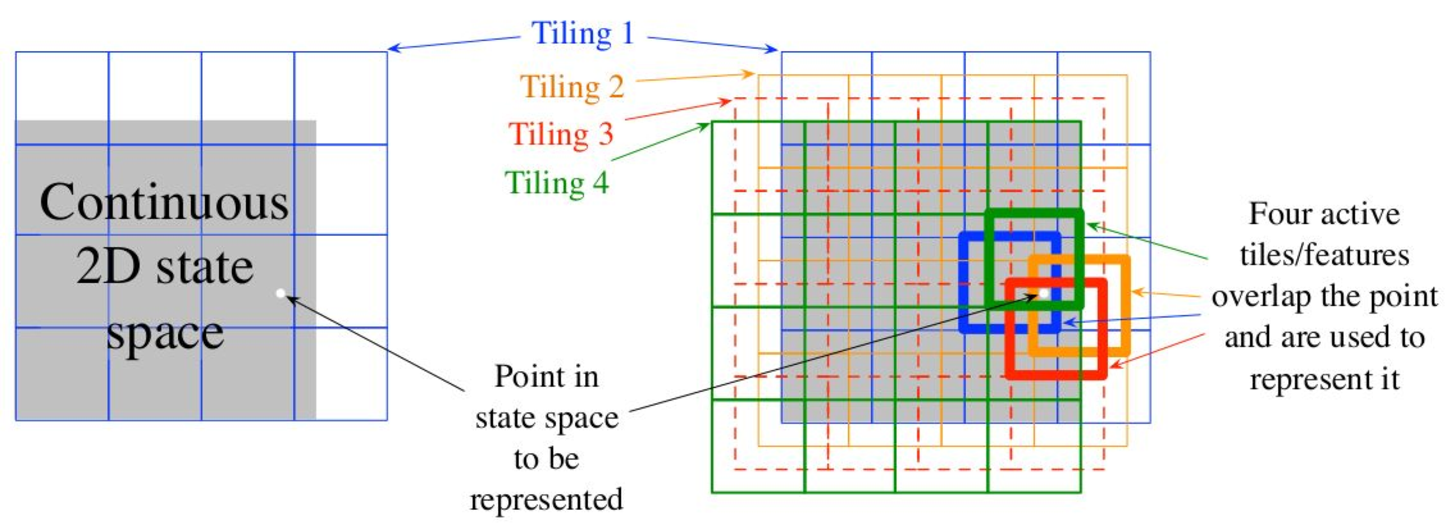
\includegraphics[keepaspectratio=true, width=1\textwidth]{\main/img/tile_coding.pdf}
    \caption[Tile Coding] {Left side: a 2-dimensional state space partitioned into a grid with 
    tiles of equal size. Right side: the same 2-dimensional space partitioned into multiple 
    tilings offset from one another by a uniform amount. Reprinted from 
    \textit{Reinforcement Learning: An Introduction} (p. 217) by \citeauthor{sutton2018}. 
    Reprinted with permission.}
    \label{fig:tile_coding}
    % Put the label *after* the caption, but inside the float
\end{figure}

How we design the feature vector \textbf{x} can have a significant impact in the performance of the algorithm.
It is also important to note that the mapping \textbf{x} does not have to be a linear as long as the inner product in equation (\ref{eq:inner_product_xtheta}) remains the same.
In this work, we will consider a popular feature extractor used in RL called \textit{tile coding} \parencite{Albus71atheory,Albus:1981:BBR:542806,sutton2018}.

In order to extract features using tile coding, the state space is partitioned on every dimension. 
For example, in two dimensions, the state space is partitioned into squares of equal size, called \textit{tiles}, such as in the left side of figure (\ref{fig:tile_coding}).
Each group of non-overlapping squares that cover the state space form a grid, also called \textit{tiling}. 
Each tile in a tiling groups all the states inside of it into the same feature, which is considered active when the current state corresponds to any of the states inside of the tile.
As a consequence we gain some generalization across states at the cost of losing some resolution.
In order to gain back some of the resolution, we can add another copy of the same tiling with a small offset so that it partially overlaps the original tiling.
By repeating this process we obtain several tilings that are slightly offset from each other, such as in the right side of figure (\ref{fig:tile_coding}).
Additionally, for action-value estimates we keep a separate set of tilings for each different action. 
The number of active features represent a vector of indexes each corresponding to an element of the parameter vector $\boldsymbol\theta_t$. 
Hence, computing the inner product in equation (\ref{eq:inner_product_xtheta}) corresponds to adding up the elements of $\boldsymbol\theta_t$ corresponding to the active features.


%%%%% Non-Linear Function Approximation: Artificial Neural Networks %%%%%%%%%%
\subsection{Non-Linear Function Approximation: Neural Networks} 

Artificial Neural Networks (ANN) are one of the most popular methods used for non-linear function approximation.
An ANN is a network of interconnected units that behave similar to the neurons in the human brain.
Additionally, ANN's can have several layers of neurons in which case we refer to them as a \textit{deep neural networks}.
The study of deep neural networks is on itself field in machine learning known as \textit{deep learning}. 

ANN's can have several layers of interconnected neurons, but, in their simplest form, they require at least three different types of layers. 
First, an input layer that represents the input observations, \textbf{x}.
The input layer is followed by one or several hidden layers with several neurons that process the information and propagate it forward.
Lastly, the network has one output layer which returns the approximated value of the function.

The information in the network is processed at every hidden and output layer by multiplying the input of the layer by the weights corresponding to each neuron and then adding a bias term.
After adding the bias term, a non-linear function $g$, also known as \textit{activation function}, is applied individually to each element of the layer and then its output is propagated forward to the next layer.
Among the most popular type of activation functions are the ReLu gate, $g(x) = \max(0,x)$, and the sigmoid function, $g(x) = \frac{1}{1+e^{-x}}$. 
Since each neuron and bias term is represented as a vector of parameters, each layer can be represented as a matrix, $\boldsymbol\theta$, of weights corresponding to the neurons and bias term, $\textbf{b}$.
Hence, for an ANN with one input layer; one hidden layer with activation function $g_1$, parameters $\boldsymbol\theta_1$, and bias term $\textbf{b}_1$; and one output layer with activation function $g_2$, parameters $\boldsymbol\theta_2$ and bias term $\textbf{b}_2$, the function, $\hat{f}$, is approximated as
%
\begin{equation}
\label{eq:ann_example}
\hat{f}(\boldsymbol{x}) = 
	g_2(\boldsymbol\theta_2^T g_1( \boldsymbol\theta_1^T \boldsymbol{x} + \textbf{b}_1) + \textbf{b}_2).
\end{equation}
%
% We can also represent an ANN graphically.
% For example, the network from equation (\ref{eq:ann_example}) can be represented as in figure (\textbf{draw network}) where every circle represents a neuron and every arrow represents weights multiplying and being added to the input of the layer.

Just as in the linear case, all the parameters from the network can be learned using SGD or semi-gradient methods in order to minimize the action-value error.
The corresponding update function is the same as in equation (\ref{eq:semi_grad_update}), but in this case the gradient is with respect with each $\boldsymbol\theta_i$ and $\textbf{b}_i$ in the network, which depend on the network architecture.
In order to compute this gradient, we use the \textit{backpropagation algorithm} \parencite{Lecun1985,Rumelhart:1986}, which is the algorithm most often used in the deep learning community.
Additionally, the gradient can be computed using a \textit{mini-batch} of observations instead of a single observation, which provide a more accurate estimate of the gradient \parencite{Goodfellow-et-al-2016}. 

Many methods have been proposed for using ANN's for estimating value functions in RL.
In this body of work we will focus on the architecture developed by \citeauthor{mnih2015humanlevel} \citeyear{mnih2015humanlevel} called Deep Q-Network (DQN). 
The DQN is a deep neural network architecture with three convolutional layers \parencite{Lecun1989} and one feed-forward layer.
The network is used to compute the action-values for Atari 2600 games from the Arcade Learning Environment \parencite{bellemare13arcade}.

The DQN architecture introduces two main modifications to RL agents. 
First, the DQN agents do not learn directly from observations collected from the environment.
Instead, agents store observations in a buffer, called \textit{experience replay buffer}, and at every timestep they collect a mini-batch of observation from the buffer to compute an update \parencite{Lin1992}.
Second, DQN agents have two separate set of weights corresponding to separate networks.
One network, called \textit{target network}, is used to compute the estimate of the return, $\hat{G}$, and is updated less frequently. 
The other network is updated at every timestep using the estimate of the return computed using the target network and the update function from equation (\ref{eq:semi_grad_update}).
In the next section, we will introduce modifications to DQN in order to adapt it to other algorithms such as $n$-step Sarsa, tree backup, and $Q(\sigma)$.

\end{document}